\documentclass{article}

% content/resources/templates/preamble.tex
\usepackage[margin=0.6in]{geometry}
\author{Milav Dabgar}
\usepackage{amsmath,amssymb,amsthm}
\usepackage{booktabs}
\usepackage{multirow}
\usepackage{xcolor}
\usepackage{tcolorbox}
\tcbuselibrary{breakable,skins}
\usepackage[colorlinks=true,linkcolor=blue]{hyperref}
\usepackage{titlesec}
\usepackage{enumitem}
\usepackage{tikz}
\usepackage{pgfplots}
\usepackage{circuitikz}
\usepackage[version=4]{mhchem}
\usepackage{longtable}
\usepackage{array}
\usepackage{float}
\usepackage{caption}
\usepackage{listings}

\lstset{
  basicstyle=\small\ttfamily,
  breaklines=true,
  breakatwhitespace=false,
  postbreak=\mbox{\textcolor{red}{$\hookrightarrow$}\space},
  float=false,
  numbers=left,
  numberstyle=\tiny\color{gray},
  numbersep=10pt,
  xleftmargin=2em,
  keywordstyle=\color{blue},
  commentstyle=\color{green!60!black},
  stringstyle=\color{purple},
  backgroundcolor=\color{gray!5},
  showstringspaces=false,
  tabsize=2,
  captionpos=b,
  keepspaces=true,
  columns=flexible
}

\pgfplotsset{compat=1.18}
\usetikzlibrary{shapes,arrows,positioning,calc,patterns,decorations.pathmorphing,decorations.markings,arrows.meta}

% Color scheme
\definecolor{headcolor}{RGB}{0,102,204}
\definecolor{keycolor}{RGB}{220,20,60}
\definecolor{solutioncolor}{RGB}{34,139,34}
\definecolor{mnemoniccolor}{RGB}{148,0,211}
\definecolor{codecolor}{RGB}{0,0,100}

% Spacing
\setlength{\parskip}{3pt}
\setlist[itemize]{nosep}
\setlist[enumerate]{nosep}

% Title formatting
\titleformat{\section}{\Large\bfseries\color{headcolor}}{\thesection}{1em}{}
\titleformat{\subsection}{\large\bfseries\color{headcolor}}{\thesubsection}{1em}{}

% Pandoc tightlist compatibility
\providecommand{\tightlist}{%
  \setlength{\itemsep}{0pt}\setlength{\parskip}{0pt}}

% Pandoc longtable compatibility
\newcounter{none}
\def\thenone{}


% content/resources/templates/english-boxes.tex

% Custom environments
\newtcolorbox{solutionbox}{
 breakable,
 enhanced,
 colback=solutioncolor!5!white,
 colframe=solutioncolor!75!black,
 fonttitle=\bfseries,
 title=Solution
}

\newtcolorbox{solutionboxnobreak}{
 colback=solutioncolor!5!white,
 colframe=solutioncolor!75!black,
 fonttitle=\bfseries,
 title=Solution
}

\newtcolorbox{keyformula}{
 breakable,
 enhanced,
 colback=keycolor!5!white,
 colframe=keycolor!75!black,
 fonttitle=\bfseries,
 title=Key Formula
}

\newtcolorbox{mnemonicboxenv}{
 breakable,
 enhanced,
 colback=mnemoniccolor!5!white,
 colframe=mnemoniccolor!75!black,
 fonttitle=\bfseries,
 title=Mnemonic
}

\newcommand{\mnemonicbox}[1]{%
  \begin{mnemonicboxenv}
    #1
  \end{mnemonicboxenv}
}


% Custom commands for GTU solutions
% This file defines semantic commands for consistent formatting

% Question command with automatic formatting
\newcommand{\question}[2]{%
  \section*{Question #1}%
  \textbf{#2}%
}

% OR question variant
\newcommand{\questionor}[2]{%
  \section*{Question #1 OR}%
  \textbf{#2}%
}

% Proper table environment with caption
\newenvironment{answertable}[1]{%
  \begin{table}[htbp]
  \centering
  \caption{#1}
}{%
  \end{table}
}

% Proper figure environment for diagrams
\newenvironment{answerdiagram}[1]{%
  \begin{figure}[htbp]
  \centering
  \caption{#1}
}{%
  \end{figure}
}

% Semantic markup for key terms
\newcommand{\keyword}[1]{\textbf{#1}}
\newcommand{\code}[1]{\texttt{#1}}
\newcommand{\classname}[1]{\texttt{#1}}
\newcommand{\methodname}[1]{\texttt{#1}}

% Proper quotation marks
\newcommand{\mnemonic}[1]{``#1''}


\title{VLSI Technology (4353206) - Summer 2025 Solution}
\date{May 19, 2025}

\begin{document}
\maketitle

\questionmarks{1(a)}{3}{Draw neat labeled diagram of physical structure of n-channel MOSFET.}

\begin{solutionbox}
\textbf{Physical Structure of n-channel MOSFET:}

\begin{center}
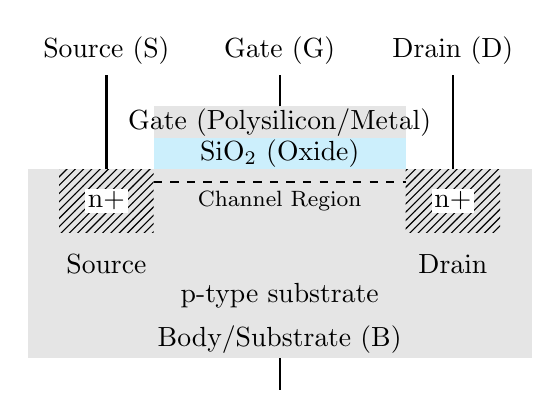
\begin{tikzpicture}[scale=0.8]
    % Substrate
    \fill[gray!20] (0,0) rectangle (8,3);
    \node at (4,1) {p-type substrate};
    \node at (4,0.3) {Body/Substrate (B)};
    \draw[thick] (4,0) -- (4,-0.5);

    % n+ regions
    \fill[pattern=north east lines] (0.5,2) rectangle (2,3);
    \node[fill=white, inner sep=1pt] at (1.25,2.5) {n+};
    \node at (1.25,1.5) {Source};
    
    \fill[pattern=north east lines] (6,2) rectangle (7.5,3);
    \node[fill=white, inner sep=1pt] at (6.75,2.5) {n+};
    \node at (6.75,1.5) {Drain};

    % Oxide
    \fill[cyan!20] (2,3) rectangle (6,3.5);
    \node at (4,3.25) {SiO$_2$ (Oxide)};

    % Gate
    \fill[black!10] (2,3.5) rectangle (6,4);
    \node at (4,3.75) {Gate (Polysilicon/Metal)};

    % Terminals
    \draw[thick] (1.25,3) -- (1.25,4.5) node[above] {Source (S)};
    \draw[thick] (6.75,3) -- (6.75,4.5) node[above] {Drain (D)};
    \draw[thick] (4,4) -- (4,4.5) node[above] {Gate (G)};

    % Channel area indication
    \draw[dashed] (2,2.8) -- (6,2.8);
    \node[font=\footnotesize] at (4,2.5) {Channel Region};
\end{tikzpicture}
\captionof{figure}{n-channel MOSFET Structure}
\end{center}

\textbf{Key Components:}
\begin{itemize}
    \item \textbf{Source}: n+ doped region providing electrons
    \item \textbf{Drain}: n+ doped region collecting electrons
    \item \textbf{Gate}: Metal electrode controlling channel
    \item \textbf{Oxide}: SiO\textsubscript{2} insulating layer
    \item \textbf{Substrate}: p-type silicon body
\end{itemize}
\end{solutionbox}

\begin{mnemonicbox}
\mnemonic{SOGD - Source, Oxide, Gate, Drain}
\end{mnemonicbox}

\questionmarks{1(b)}{4}{Draw energy band diagram of depletion and inversion of MOS under external bias with MOS biasing diagram. Explain inversion region in detail.}

\begin{solutionbox}
\textbf{MOS Biasing Circuit:}

\begin{center}
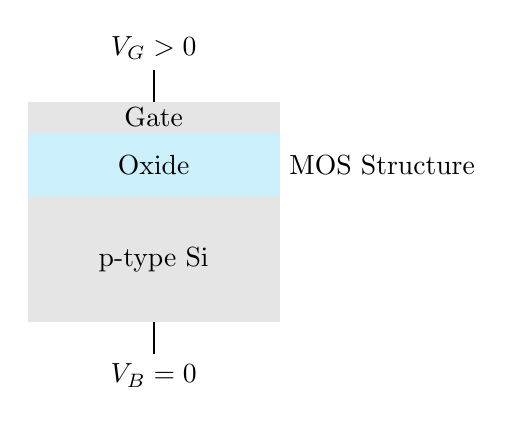
\begin{tikzpicture}[scale=0.8]
    \fill[gray!20] (0,0) rectangle (4,2);
    \node at (2,1) {p-type Si};
    \fill[cyan!20] (0,2) rectangle (4,3);
    \node at (2,2.5) {Oxide};
    \fill[black!10] (0,3) rectangle (4,3.5);
    \node at (2,3.25) {Gate};
    
    \draw[thick] (2,3.5) -- (2,4) node[above] {$V_G > 0$};
    \draw[thick] (2,0) -- (2,-0.5) node[below] {$V_B = 0$};
    
    \node[right] at (4,2.5) {MOS Structure};
\end{tikzpicture}
\captionof{figure}{MOS Biasing}
\end{center}

\textbf{Energy Band Diagrams:}

\begin{center}
\begin{tabulary}{\linewidth}{|C|C|}
\hline
\textbf{Depletion} & \textbf{Inversion} \\
\hline
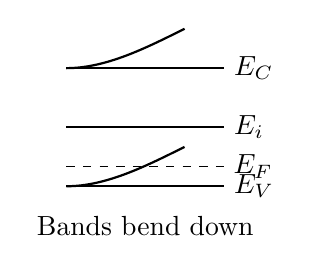
\begin{tikzpicture}[scale=0.5]
    % Depletion Bands
    \draw[thick] (0,0) -- (4,0) node[right] {$E_V$};
    \draw[thick] (0,3) -- (4,3) node[right] {$E_C$};
    \draw[dashed] (0,0.5) -- (4,0.5) node[right] {$E_F$};
    \draw[thick] (0,1.5) -- (4,1.5) node[right] {$E_i$};
    
    % Bending up
    \draw[thick] (0,0) .. controls (1,0) and (2,0.5) .. (3,1);
    \draw[thick] (0,3) .. controls (1,3) and (2,3.5) .. (3,4);
    
    \node at (2,-1) {Bands bend down};
\end{tikzpicture}
&
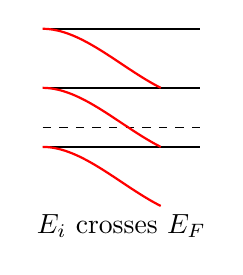
\begin{tikzpicture}[scale=0.5]
    % Inversion Bands
    \draw[thick] (0,0) -- (4,0); % Ev
    \draw[thick] (0,3) -- (4,3); % Ec
    \draw[dashed] (0,0.5) -- (4,0.5); % Ef
    \draw[thick] (0,1.5) -- (4,1.5); % Ei
    
    % Strong bending
    \draw[thick, red] (0,0) .. controls (1,0) and (2,-1) .. (3,-1.5);
    \draw[thick, red] (0,3) .. controls (1,3) and (2,2) .. (3,1.5);
    \draw[thick, red] (0,1.5) .. controls (1,1.5) and (2,0.5) .. (3,0);
    
    \node at (2,-2) {$E_i$ crosses $E_F$};
\end{tikzpicture}
\\
\hline
\end{tabulary}
\end{center}

\textbf{Inversion Region Details:}
\begin{itemize}
    \item \textbf{Strong inversion}: $V_G > V_T$ (threshold voltage)
    \item \textbf{Electron channel}: Forms at Si-SiO\textsubscript{2} interface as minority carriers (electrons) accumulate.
    \item \textbf{Channel conductivity}: Increases with gate voltage.
    \item \textbf{Threshold condition}: Surface potential $\phi_s = 2\phi_F$.
\end{itemize}
\end{solutionbox}

\begin{mnemonicbox}
\mnemonic{DIVE - Depletion, Inversion, Voltage, Electrons}
\end{mnemonicbox}

\questionmarks{1(c)}{7}{Explain I-V characteristics of MOSFET.}

\begin{solutionbox}
\textbf{I-V Characteristic Regions:}

\begin{center}
\captionof{table}{Operating Regions}
\begin{tabulary}{\linewidth}{|L|L|L|}
\hline
\textbf{Region} & \textbf{Condition} & \textbf{Drain Current ($I_D$)} \\ \hline
\textbf{Cutoff} & $V_{GS} < V_T$ & $I_D \approx 0$ \\ \hline
\textbf{Linear} & $V_{GS} > V_T, V_{DS} < V_{GS}-V_T$ & $I_D = \mu_n C_{ox} \frac{W}{L} [(V_{GS}-V_T)V_{DS} - \frac{V_{DS}^2}{2}]$ \\ \hline
\textbf{Saturation} & $V_{GS} > V_T, V_{DS} \ge V_{GS}-V_T$ & $I_D = \frac{1}{2} \mu_n C_{ox} \frac{W}{L} (V_{GS}-V_T)^2$ \\ \hline
\end{tabulary}
\end{center}

\textbf{Characteristic Curve:}

\begin{center}
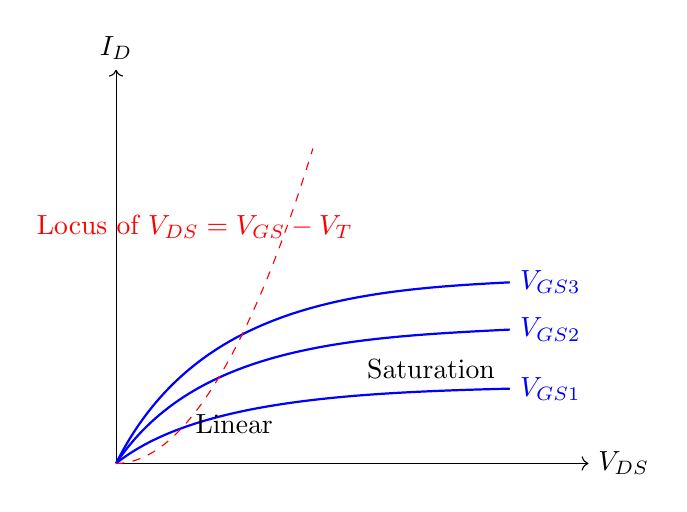
\begin{tikzpicture}[scale=1]
    \draw[->] (0,0) -- (6,0) node[right] {$V_{DS}$};
    \draw[->] (0,0) -- (0,5) node[above] {$I_D$};
    
    % Curves
    \draw[thick, blue] (0,0) .. controls (1,2) and (3,2.2) .. (5,2.3) node[right] {$V_{GS3}$};
    \draw[thick, blue] (0,0) .. controls (1,1.5) and (3,1.6) .. (5,1.7) node[right] {$V_{GS2}$};
    \draw[thick, blue] (0,0) .. controls (1,0.8) and (3,0.9) .. (5,0.95) node[right] {$V_{GS1}$};
    
    % Parabola separating regions
    \draw[dashed, red] (0,0) parabola (2.5,4);
    \node[red] at (1,3) {Locus of $V_{DS} = V_{GS}-V_T$};
    
    \node at (1.5,0.5) {Linear};
    \node at (4,1.2) {Saturation};
\end{tikzpicture}
\captionof{figure}{MOSFET I-V Characteristics}
\end{center}

\textbf{Key Parameters:}
\begin{itemize}
    \item \textbf{$\mu_n$}: Electron mobility
    \item \textbf{$C_{ox}$}: Gate oxide capacitance per unit area
    \item \textbf{$W/L$}: Channel Width to Length ratio
    \item \textbf{$V_T$}: Threshold voltage
\end{itemize}
\end{solutionbox}

\begin{mnemonicbox}
\mnemonic{CLS - Cutoff, Linear, Saturation}
\end{mnemonicbox}

\questionmarks{1(c) OR}{7}{Define scaling. Explain the need of scaling. List and explain the negative effects of scaling.}

\begin{solutionbox}
\textbf{Definition:}
\textbf{Scaling} is the systematic reduction of MOSFET dimensions to improve performance and density.

\textbf{Need for Scaling:}
\begin{itemize}
    \item \textbf{Higher Density}: More transistors per chip area, following Moore's Law.
    \item \textbf{Faster Speed}: Reduced channel length reduces carrier transit time ($t = L^2/\mu V$).
    \item \textbf{Lower Power}: Smaller parasitic capacitances decrease switching energy.
    \item \textbf{Cost Reduction}: More chips per wafer reduces cost per die.
\end{itemize}

\textbf{Scaling Types:}

\begin{center}
\captionof{table}{Scaling Strategies}
\begin{tabulary}{\linewidth}{|L|C|C|C|}
\hline
\textbf{Type} & \textbf{Gate Length} & \textbf{Supply Voltage} & \textbf{Oxide Thickness} \\ \hline
\textbf{Constant Voltage} & $\downarrow \alpha$ & Constant & $\downarrow \alpha$ \\ \hline
\textbf{Constant Field} & $\downarrow \alpha$ & $\downarrow \alpha$ & $\downarrow \alpha$ \\ \hline
\end{tabulary}
\end{center}

\textbf{Negative Effects:}
\begin{itemize}
    \item \textbf{Short Channel Effects (SCE)}: $V_T$ roll-off and drain-induced barrier lowering (DIBL).
    \item \textbf{Hot Carrier Effects}: High electric fields near drain inject carriers into oxide, degrading device.
    \item \textbf{Gate Leakage}: Thin oxide leads to quantum tunneling current.
    \item \textbf{Process Variations}: Difficulty in controlling dimensions at nano-scale.
    \item \textbf{Power Density}: Increased heat per unit area creates thermal management issues.
\end{itemize}
\end{solutionbox}

\begin{mnemonicbox}
\mnemonic{SHGPP - Short channel, Hot carrier, Gate leakage, Process, Power}
\end{mnemonicbox}

\questionmarks{2(a)}{3}{Implement Y' = (AB' + A'B) using CMOS.}

\begin{solutionbox}
\textbf{Logic Analysis:}
$Y' = AB' + A'B = A \oplus B$ (XOR function).

\textbf{CMOS Implementation:}

\begin{center}
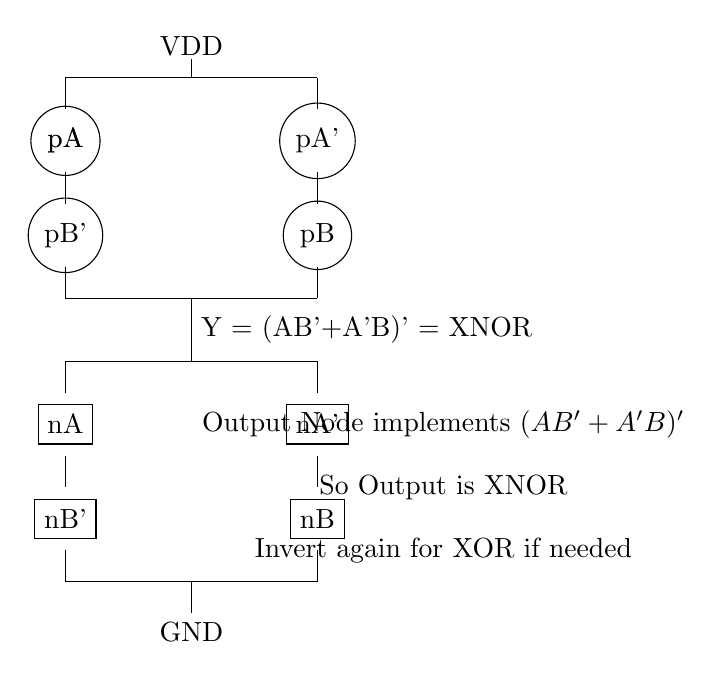
\begin{tikzpicture}[scale=0.8]
    % PMOS Network (Pull-up for XOR is complex, usually implemented as AOI or transmission gates. 
    % But for straight CMOS: Y = (A XOR B)' = XNOR. Wait, question asks for Y' = XOR. So Y = XNOR.
    % To implement Y' = XOR directly, we usually implement Y = XNOR and take output from there? 
    % Or Y' is the function itself? "Implement Y' = ..." implies Output is Y'.
    % CMOS naturally inverts. To get XOR, inputs to Pull Down should implement XOR. Pull Up implements XNOR.
    % Pull Down (NMOS) for XOR: (A and B') OR (A' and B) -> Parallel branches of series pairs.
    % Pull Up (PMOS) for XOR: Dual of PD.
    
    % VDD
    \node at (4,6) {VDD};
    \draw (4,5.8) -- (4,5.5);
    \draw (2,5.5) -- (6,5.5);
    
    % PMOS (Dual of AB' + A'B => (A'+B)(A+B'))
    % Left branch: A' in series with B
    % Right branch: A in series with B'
    % Actually: (A+B')(A'+B) = AA' + AB + A'B' + BB' = AB + A'B'. This is XNOR.
    % So PMOS implements XNOR logic.
    
    % Left PMOS branch
    \draw (2,5.5) -- (2,5);
    \node[draw,circle,minimum size=0.5cm] (p1) at (2,4.5) {pA}; % pA is PMOS with input A
    \node[draw,circle,white] at (2,4.5) {A}; \node at (2,4.5) {pA};
    \draw (2,4) -- (2,3.5);
    \node[draw,circle,minimum size=0.5cm] (p2) at (2,3) {pB'};
    \draw (2,2.5) -- (2,2);
    
    % Right PMOS branch
    \draw (6,5.5) -- (6,5);
    \node[draw,circle,minimum size=0.5cm] (p3) at (6,4.5) {pA'};
    \draw (6,4) -- (6,3.5);
    \node[draw,circle,minimum size=0.5cm] (p4) at (6,3) {pB};
    \draw (6,2.5) -- (6,2);
    
    \draw (2,2) -- (6,2);
    \draw (4,2) -- (4,1.5) node[right] {Y = (AB'+A'B)' = XNOR}; 
    
    % Wait, question asks Y' = AB' + A'B. So Output = Y' ? 
    % If Output node implies Y', then Pull Down logic is (AB' + A'B). 
    % And Pull Up is dual.
    % Let's draw Pull Down as AB' + A'B
    
    \draw (4,1.5) -- (4,1);
    \draw (2,1) -- (6,1);
    
    % NMOS Left: A series B'
    \draw (2,1) -- (2,0.5);
    \node[draw,rectangle,minimum size=0.5cm] (n1) at (2,0) {nA};
    \draw (2,-0.5) -- (2,-1);
    \node[draw,rectangle,minimum size=0.5cm] (n2) at (2,-1.5) {nB'};
    \draw (2,-2) -- (2,-2.5);
    
    % NMOS Right: A' series B
    \draw (6,1) -- (6,0.5);
    \node[draw,rectangle,minimum size=0.5cm] (n3) at (6,0) {nA'};
    \draw (6,-0.5) -- (6,-1);
    \node[draw,rectangle,minimum size=0.5cm] (n4) at (6,-1.5) {nB};
    \draw (6,-2) -- (6,-2.5);
    
    \draw (2,-2.5) -- (6,-2.5);
    \draw (4,-2.5) -- (4,-3) node[below] {GND};
    
    \node at (8,0) {Output Node implements $(AB' + A'B)'$};
    \node at (8,-1) {So Output is XNOR};
    \node at (8,-2) {Invert again for XOR if needed};
\end{tikzpicture}
\captionof{figure}{Static CMOS Implementation for XNOR (inverted XOR)}
\end{center}
\textit{Note: The circuit above implements $(AB' + A'B)'$. To get $Y' = AB' + A'B$, we technically need an inverter at the output, or this represents the structure where pull-down matches the expression.}
\end{solutionbox}

\begin{mnemonicbox}
\mnemonic{XOR needs complementary switching}
\end{mnemonicbox}

\questionmarks{2(b)}{4}{Explain enhancement load inverter with its circuit diagrams.}

\begin{solutionbox}
\textbf{Circuit Diagram:}

\begin{center}
\begin{tikzpicture}[scale=1]
    \node at (0,4) {VDD};
    \draw (0,3.8) -- (0,3.5);
    
    % Load Transistor (Enhancement NMOS) - Gate to VDD or VGG
    % Usually Saturated Enhancement Load has Gate to Drain (Diode connected)
    % Or Linear Enhancement Load has Gate to separate bias VDD+Vt.
    % "Enhancement load" usually implies Saturated (Gate tied to Drain/VDD)
    
    \draw (0,3.5) -- (0,3); % Drain
    \draw (-0.5,2.5) -- (0.5,2.5); % Gate
    \draw (0,2) -- (0,1.5); % Source
    
    % NMOS symbol details
    \draw (0,3) -- (0,2);
    \node at (0.8,2.5) {ML (Load)};
    
    % Connection Gate to Drain (Saturated)
    \draw (-0.5,2.5) -- (-0.5,3.2) -- (0,3.2);
    
    \draw (0,1.5) -- (2,1.5) node[right] {$V_{out}$};
    
    % Driver Transistor
    \draw (0,1.5) -- (0,1);
    \draw (-0.5,0.5) -- (0.5,0.5); % Gate
    \draw (0,0) -- (0,-0.5); % Source
    \draw (0,1) -- (0,0);
    \node at (0.8,0.5) {MD (Driver)};
    
    \draw (-0.5,0.5) -- (-1,0.5) node[left] {$V_{in}$};
    \draw (0,-0.5) -- (0,-1) node[below] {GND};
\end{tikzpicture}
\captionof{figure}{Saturated Enhancement Load Inverter}
\end{center}

\textbf{Configuration:}
\begin{itemize}
    \item \textbf{Load (ML)}: Enhancement NMOS with Gate connected to Drain ($V_{GS} = V_{DS}$). Always in Saturation or Cutoff.
    \item \textbf{Driver (MD)}: Enhancement NMOS with Gate as input.
\end{itemize}

\textbf{Operation:}
\begin{itemize}
    \item \textbf{High Output ($V_{OH}$)}: Limited to $V_{DD} - V_T$ because load turns off when $V_{out}$ rises to that level.
    \item \textbf{Low Output ($V_{OL}$)}: Close to 0V (depends on ratio $K_D/K_L$).
    \item \textbf{Disadvantage}: Degraded logic high ($V_{DD} - V_T$) and continuous power dissipation when $V_{in}$ is high.
\end{itemize}
\end{solutionbox}

\begin{mnemonicbox}
\mnemonic{ELI - Enhancement Load Inverter has threshold Issues}
\end{mnemonicbox}

\questionmarks{2(c)}{7}{Explain Voltage Transfer Characteristic of inverter.}

\begin{solutionbox}
\textbf{VTC Curve:}

\begin{center}
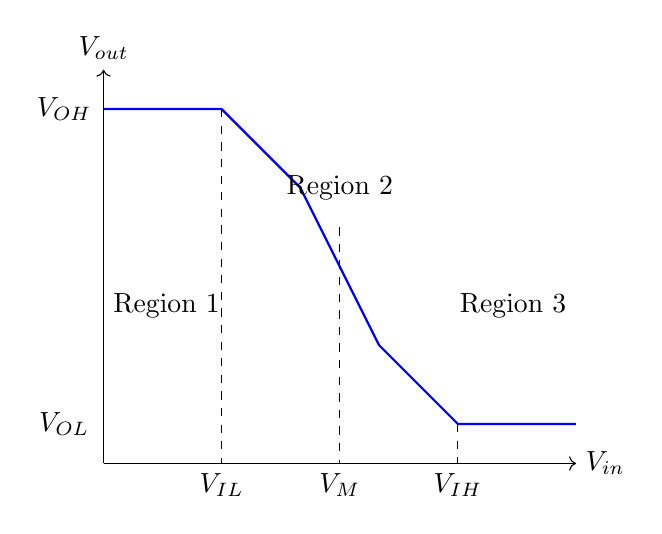
\begin{tikzpicture}[scale=1]
    \draw[->] (0,0) -- (6,0) node[right] {$V_{in}$};
    \draw[->] (0,0) -- (0,5) node[above] {$V_{out}$};
    
    \node at (-0.5, 4.5) {$V_{OH}$};
    \node at (-0.5, 0.5) {$V_{OL}$};
    
    % VTC Shape
    \draw[thick, blue] (0,4.5) -- (1.5,4.5) -- (2.5,3.5) -- (3.5,1.5) -- (4.5,0.5) -- (6,0.5);
    
    % Points
    \draw[dashed] (1.5,4.5) -- (1.5,0) node[below] {$V_{IL}$};
    \draw[dashed] (4.5,0.5) -- (4.5,0) node[below] {$V_{IH}$};
    \draw[dashed] (3,3) -- (3,0) node[below] {$V_M$};
    
    \node at (0.8, 2) {Region 1};
    \node at (3, 3.5) {Region 2};
    \node at (5.2, 2) {Region 3};
\end{tikzpicture}
\captionof{figure}{Ideally Inverter VTC}
\end{center}

\textbf{Key Parameters:}
\begin{center}
\begin{tabulary}{\linewidth}{|L|L|L|}
\hline
\textbf{Parameter} & \textbf{Description} & \textbf{Ideal Value} \\ \hline
\textbf{$V_{OH}$} & Output High Voltage & $V_{DD}$ \\ \hline
\textbf{$V_{OL}$} & Output Low Voltage & $0V$ \\ \hline
\textbf{$V_{IH}$} & Input High Voltage & $\approx V_{DD}/2$ \\ \hline
\textbf{$V_{IL}$} & Input Low Voltage & $\approx V_{DD}/2$ \\ \hline
\textbf{$V_M$} & Switching Threshold & $V_{DD}/2$ \\ \hline
\end{tabulary}
\end{center}

\textbf{Noise Margins:}
\begin{itemize}
    \item $NM_H = V_{OH} - V_{IH}$ (High noise margin)
    \item $NM_L = V_{IL} - V_{OL}$ (Low noise margin)
\end{itemize}

\textbf{Regions:}
\begin{itemize}
    \item \textbf{Region 1}: $V_{in}$ low, $V_{out}$ high (PMOS Linear, NMOS Cutoff)
    \item \textbf{Region 2}: Transition region (Both Saturation)
    \item \textbf{Region 3}: $V_{in}$ high, $V_{out}$ low (PMOS Saturation, NMOS Linear)
\end{itemize}
\end{solutionbox}

\begin{mnemonicbox}
\mnemonic{VTC shows VOICE - VOH, VOL, Input thresholds, Characteristics, Everything}
\end{mnemonicbox}

\questionmarks{2(a) OR}{3}{Explain NAND2 gate using CMOS.}

\begin{solutionbox}
\textbf{CMOS NAND2 Circuit:}

\begin{center}
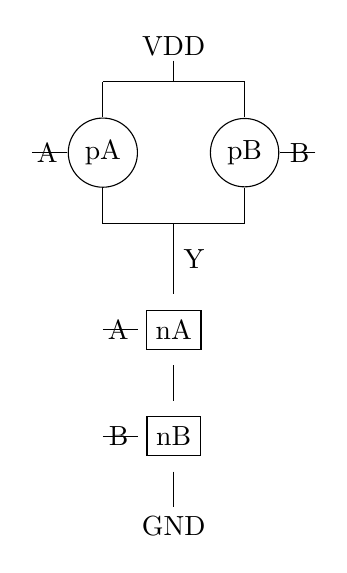
\begin{tikzpicture}[scale=0.9]
    \node at (2,5) {VDD};
    \draw (2,4.8) -- (2,4.5);
    
    % PMOS Parallel
    \draw (1,4.5) -- (3,4.5);
    
    \draw (1,4.5) -- (1,4);
    \node[draw,circle,minimum size=0.5cm] (p1) at (1,3.5) {pA};
    \draw (0,3.5) -- (0.5,3.5) node[left] {A};
    \draw (1,3) -- (1,2.5);
    
    \draw (3,4.5) -- (3,4);
    \node[draw,circle,minimum size=0.5cm] (p2) at (3,3.5) {pB};
    \draw (4,3.5) -- (3.5,3.5) node[right] {B};
    \draw (3,3) -- (3,2.5);
    
    \draw (1,2.5) -- (3,2.5);
    \draw (2,2.5) -- (2,2) node[right] {Y};
    
    % NMOS Series
    \draw (2,2) -- (2,1.5);
    \node[draw,rectangle,minimum size=0.5cm] (n1) at (2,1) {nA};
    \draw (1,1) -- (1.5,1) node[left] {A};
    \draw (2,0.5) -- (2,0);
    \node[draw,rectangle,minimum size=0.5cm] (n2) at (2,-0.5) {nB};
    \draw (1,-0.5) -- (1.5,-0.5) node[left] {B};
    \draw (2,-1) -- (2,-1.5) node[below] {GND};
\end{tikzpicture}
\captionof{figure}{CMOS NAND2 Gate}
\end{center}

\textbf{Operation:}
\begin{itemize}
    \item \textbf{Pull-Up Network}: PMOS inputs A and B in parallel. If A=0 OR B=0, output pulled to VDD.
    \item \textbf{Pull-Down Network}: NMOS inputs A and B in series. Only if A=1 AND B=1, output pulled to GND.
\end{itemize}

\textbf{Truth Table:}
\begin{center}
\begin{tabulary}{0.5\linewidth}{|C|C|C|}
\hline
\textbf{A} & \textbf{B} & \textbf{Y} \\ \hline
0 & 0 & 1 \\ \hline
0 & 1 & 1 \\ \hline
1 & 0 & 1 \\ \hline
1 & 1 & 0 \\ \hline
\end{tabulary}
\end{center}
\end{solutionbox}

\begin{mnemonicbox}
\mnemonic{NAND - Not AND, Parallel PMOS, Series NMOS}
\end{mnemonicbox}

\questionmarks{2(b) OR}{4}{Explain operating mode and VTC of Resistive load inverter circuit.}

\begin{solutionbox}
\textbf{Circuit Configuration:}

\begin{center}
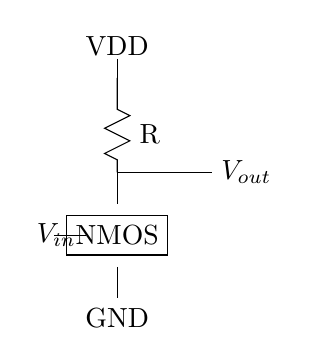
\begin{tikzpicture}[scale=0.8]
    \node at (0,3.5) {VDD};
    \draw (0,3.3) -- (0,3);
    
    \draw (0,3) -- (0,2.5) -- (0.2,2.4) -- (-0.2,2.2) -- (0.2,2.0) -- (-0.2,1.8) -- (0,1.7) -- (0,1.5);
    \node[right] at (0.2, 2.1) {R};
    
    \draw (0,1.5) -- (1.5,1.5) node[right] {$V_{out}$};
    \draw (0,1.5) -- (0,1);
    
    \node[draw,rectangle,minimum size=0.5cm] (n1) at (0,0.5) {NMOS};
    \draw (-1,0.5) -- (-0.5,0.5) node[left] {$V_{in}$};
    
    \draw (0,0) -- (0,-0.5) node[below] {GND};
\end{tikzpicture}
\captionof{figure}{Resistive Load Inverter}
\end{center}

\textbf{Operating Modes:}
\begin{itemize}
    \item \textbf{$V_{in} = 0$ (Low)}: NMOS OFF. $V_{out} = V_{DD}$.
    \item \textbf{$V_{in} = V_{DD}$ (High)}: NMOS ON (Linear). $V_{out} = V_{VOL}$.
    \item \textbf{$V_{OL}$ Calculation}: $V_{OL} = \frac{R_{ON}}{R_{ON} + R} V_{DD}$.
\end{itemize}

\textbf{Design Trade-offs:}
\begin{itemize}
    \item \textbf{Large R}: Better $V_{OL}$, lower power, but slower switching (high RC delay).
    \item \textbf{Small R}: Faster switching, but poor $V_{OL}$ and high power consumption.
    \item \textbf{Area}: Resistors consume significant silicon area compared to transistors.
\end{itemize}
\end{solutionbox}

\begin{mnemonicbox}
\mnemonic{RLI - Resistive Load has Inevitable power consumption}
\end{mnemonicbox}

% ... Continuing with Q2(c) OR ...

\questionmarks{2(c) OR}{7}{Draw CMOS inverter and explain its operation with VTC.}

\begin{solutionbox}
\textbf{CMOS Inverter Circuit:}

\begin{center}
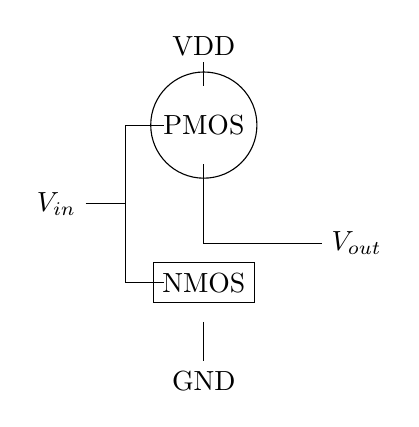
\begin{tikzpicture}[scale=1]
    \node at (0,3.5) {VDD};
    \draw (0,3.3) -- (0,3);
    \node[draw,circle,minimum size=0.5cm] (p1) at (0,2.5) {PMOS};
    \draw (0,2) -- (0,1) -- (1.5,1) node[right] {$V_{out}$};
    \node[draw,rectangle,minimum size=0.5cm] (n1) at (0,0.5) {NMOS};
    \draw (0,0) -- (0,-0.5) node[below] {GND};
    
    % Input line
    \draw (-1.5,1.5) node[left] {$V_{in}$} -- (-1,1.5);
    \draw (-1,1.5) -- (-1,2.5) -- (-0.5,2.5); % To PMOS gate
    \draw (-1,1.5) -- (-1,0.5) -- (-0.5,0.5); % To NMOS gate
\end{tikzpicture}
\captionof{figure}{CMOS Inverter}
\end{center}

\textbf{Operation Regions:}
\begin{center}
\begin{tabulary}{\linewidth}{|L|C|C|L|L|}
\hline
\textbf{$V_{in}$ Range} & \textbf{PMOS} & \textbf{NMOS} & \textbf{$V_{out}$} & \textbf{Region} \\ \hline
$0$ to $V_{TN}$ & ON & OFF & $V_{DD}$ & 1 \\ \hline
$V_{TN}$ to $V_{DD}-|V_{TP}|$ & ON & ON & Transition & 2 \\ \hline
$V_{DD}-|V_{TP}|$ to $V_{DD}$ & OFF & ON & $0V$ & 3 \\ \hline
\end{tabulary}
\end{center}

\textbf{VTC Analysis:}
The VTC is nearly ideal square-like.
\begin{itemize}
    \item \textbf{Region 1}: Output pulled hard to VDD.
    \item \textbf{Region 2}: Both transistors in saturation (shortly) causing steep drop. Gain is very high.
    \item \textbf{Region 3}: Output pulled hard to GND.
\end{itemize}

\textbf{Key Features:}
\begin{itemize}
    \item \textbf{Zero Static Power}: In steady states (high/low), one transistor is always OFF.
    \item \textbf{Rail-to-Rail Swing}: Logic levels are exact VDD and GND.
    \item \textbf{Symmetric Design}: If $\beta_n = \beta_p$, switching threshold $V_M = V_{DD}/2$.
\end{itemize}
\end{solutionbox}

\begin{mnemonicbox}
\mnemonic{CMOS has Zero Static Power with Full Swing}
\end{mnemonicbox}

\questionmarks{3(a)}{3}{Realize $Y= (\overline{A}+\overline{B})\overline{C}+\overline{D}+\overline{E}$ using depletion load.}

\begin{solutionbox}
\textbf{Logic Simplification:}
$Y = (\bar{A}+\bar{B})\bar{C}+\bar{D}+\bar{E}$
Wait, let's check exact expression: $Y = (\bar{A}+\bar{B})\bar{C}+\bar{D}+\bar{E}$. This looks like sum of products.
Depletion load implies NMOS logic. Y is the output of proper logic.
Usually we implement the complement in Pull Down.
Complement of Y?
If Y is the target, and we use NMOS with Depletion load (which is basically an inverter structure for the logic block), the Pull Down network should minimize $\bar{Y}$.
$\bar{Y} = \overline{(\bar{A}+\bar{B})\bar{C}+\bar{D}+\bar{E}} = \overline{(\bar{A}+\bar{B})\bar{C}} \cdot \overline{\bar{D}} \cdot \overline{\bar{E}}$.
$\bar{Y} = \overline{(\bar{A}+\bar{B})\bar{C}} \cdot D \cdot E$
$= ( \overline{\bar{A}+\bar{B}} + \overline{\bar{C}} ) \cdot D \cdot E = (AB + C)DE = ABDE + CDE$.

This seems complex. Let's assume the question implies implementing the function directly as written using "Depletion Load NMOS Logic".
Standard NMOS logic implements NOR/NAND inherently.
Output $F = \overline{PDN}$.
So if we want Output Y, we need PDN function equal to $\bar{Y}$.
Let's re-read: "Realize Y=..".
Usually implies: Design a gate where Output is Y.
So PDN must implement $\bar{Y}$.
If $\bar{Y} = ABDE + CDE = (AB+C)DE$.
PDN: D and E in series with (C parallel (A series B)).

\textbf{Depletion Load Implementation:}

\begin{center}
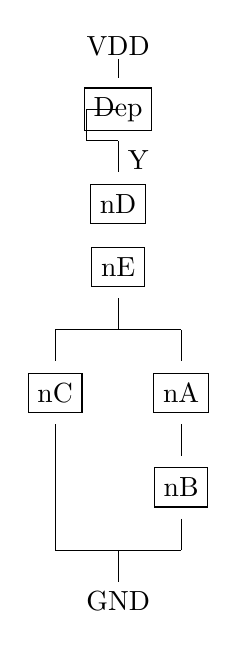
\begin{tikzpicture}[scale=0.8]
    \node at (0,4) {VDD};
    \draw (0,3.8) -- (0,3.5);
    
    % Depletion Load
    \node[draw,rectangle,minimum size=0.5cm] (load) at (0,3) {Dep};
    \draw (-0.5,3) -- (0,3); % Gate to Source/Output
    \draw (-0.5,3) -- (-0.5,2.5) -- (0,2.5);
    
    \draw (0,2.5) -- (0,2);
    \node[right] at (0,2.2) {Y};
    
    % PDN implements (AB+C)DE
    % Series D, Series E, then (Parallel C, Series A-B)
    
    \node[draw,rectangle,minimum size=0.5cm] (nD) at (0,1.5) {nD};
    \node[draw,rectangle,minimum size=0.5cm] (nE) at (0,0.5) {nE};
    
    % Below E, split into C and A-B
    \draw (0,0) -- (0,-0.5);
    \draw (-1,-0.5) -- (1,-0.5);
    
    % Left branch C
    \draw (-1,-0.5) -- (-1,-1);
    \node[draw,rectangle,minimum size=0.5cm] (nC) at (-1,-1.5) {nC};
    \draw (-1,-2) -- (-1,-2.5);
    
    % Right branch A-B
    \draw (1,-0.5) -- (1,-1);
    \node[draw,rectangle,minimum size=0.5cm] (nA) at (1,-1.5) {nA};
    \draw (1,-2) -- (1,-2.5);
    \node[draw,rectangle,minimum size=0.5cm] (nB) at (1,-3) {nB};
    \draw (1,-3.5) -- (1,-4);
    
    \draw (-1,-2.5) -- (-1,-4);
    \draw (-1,-4) -- (1,-4);
    \draw (0,-4) -- (0,-4.5) node[below] {GND};
\end{tikzpicture}
\captionof{figure}{Depletion Load Logic for Y}
\end{center}
\end{solutionbox}

\begin{mnemonicbox}
\mnemonic{Depletion Load with Parallel/Series pull-down Paths}
\end{mnemonicbox}

\questionmarks{3(b)}{4}{Write a short note on FPGA.}

\begin{solutionbox}
\textbf{FPGA Definition:}
\textbf{Field Programmable Gate Array} - A reconfigurable integrated circuit that can be programmed by the customer after manufacturing.

\textbf{Architecture Components:}
\begin{itemize}
    \item \textbf{CLB (Configurable Logic Block)}: Basic logic unit (LUTs, Flip-flops).
    \item \textbf{IOB (Input/Output Block)}: Interface with external pins.
    \item \textbf{Interconnects}: Programmable routing channels (Vertical/Horizontal).
    \item \textbf{Switch Matrix}: Programmable connections between routing tracks.
\end{itemize}

\textbf{Programming Technologies:}
\begin{itemize}
    \item \textbf{SRAM-based}: Volatile, fast reconfiguration, high density.
    \item \textbf{Antifuse}: Non-volatile, one-time programmable, secure.
    \item \textbf{Flash-based}: Non-volatile, reprogrammable.
\end{itemize}

\textbf{Advantages vs ASIC:}
\begin{itemize}
    \item \textbf{Flexibility}: Can be updated/fixed post-deployment.
    \item \textbf{Time-to-market}: No physical fabrication wait time.
    \item \textbf{Cost}: Low NRE (Non-Recurring Engineering) cost, good for low volume.
\end{itemize}
\end{solutionbox}

\begin{mnemonicbox}
\mnemonic{FPGA - Flexible Programming Gives Advantages}
\end{mnemonicbox}

\questionmarks{3(c)}{7}{Draw and explain Y chart design flow.}

\begin{solutionbox}
\textbf{Y-Chart Diagram:}

\begin{center}
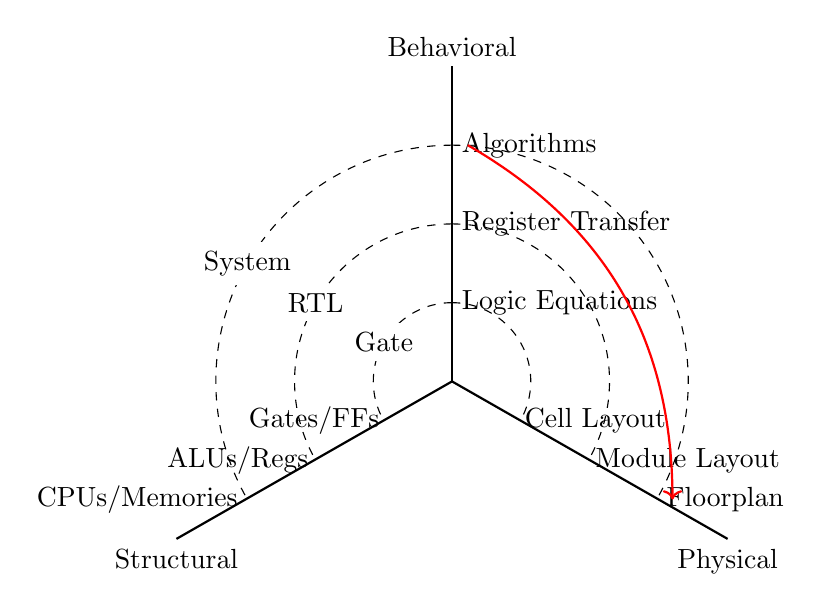
\begin{tikzpicture}[scale=1]
    % Axes
    \draw[thick] (0,0) -- (0,4) node[above] {Behavioral};
    \draw[thick] (0,0) -- (-3.5,-2) node[below] {Structural};
    \draw[thick] (0,0) -- (3.5,-2) node[below] {Physical};
    
    % Circles/Arcs for levels
    % System
    \draw[dashed] (0,3) arc (90:210:3) node[midway, fill=white] {System};
    \draw[dashed] (0,3) arc (90:-30:3);
    
    % Register Transfer
    \draw[dashed] (0,2) arc (90:210:2) node[midway, fill=white] {RTL};
    \draw[dashed] (0,2) arc (90:-30:2);
    
    % Logic
    \draw[dashed] (0,1) arc (90:210:1) node[midway, fill=white] {Gate};
    \draw[dashed] (0,1) arc (90:-30:1);
    
    % Labels
    \node[anchor=west] at (0,3) {Algorithms};
    \node[anchor=west] at (0,2) {Register Transfer};
    \node[anchor=west] at (0,1) {Logic Equations};
    
    \node[anchor=east] at (-2.6,-1.5) {CPUs/Memories};
    \node[anchor=east] at (-1.7,-1) {ALUs/Regs};
    \node[anchor=east] at (-0.8,-0.5) {Gates/FFs};
    
    \node[anchor=west] at (2.6,-1.5) {Floorplan};
    \node[anchor=west] at (1.7,-1) {Module Layout};
    \node[anchor=west] at (0.8,-0.5) {Cell Layout};
    
    % Spiral flow
    \draw[->, red, thick] (0.2,3) to[bend left] (2.8,-1.5);
\end{tikzpicture}
\captionof{figure}{Gajski-Kuhn Y-Chart}
\end{center}

\textbf{Design Domains:}
\begin{itemize}
    \item \textbf{Behavioral}: Describes \textit{what} simple system does (Algorithms, Equations).
    \item \textbf{Structural}: Describes \textit{how} components are connected (Netlists, Gates).
    \item \textbf{Physical}: Describes \textit{where} components are placed (Layout, Geometry).
\end{itemize}

\textbf{Abstraction Levels:}
\begin{itemize}
    \item \textbf{System Level}: High level architectural blocks.
    \item \textbf{RTL}: Data flow between registers.
    \item \textbf{Gate Level}: Boolean logic implementation.
    \item \textbf{Transistor/Layout Level}: Physical device details.
\end{itemize}
\end{solutionbox}

\begin{mnemonicbox}
\mnemonic{Y-Chart: Behavioral, Structural, Physical - BSP domains}
\end{mnemonicbox}

\questionmarks{3(a) OR}{3}{Explain NOR2 gate using depletion load.}

\begin{solutionbox}
\textbf{Depletion Load NOR2 Circuit:}

\begin{center}
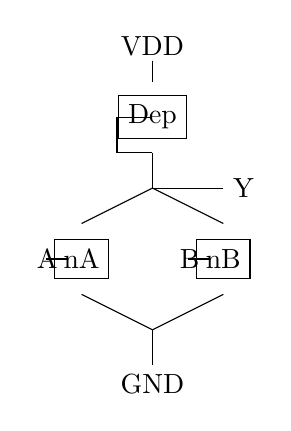
\begin{tikzpicture}[scale=0.9]
    \node at (0,4) {VDD};
    \draw (0,3.8) -- (0,3.5);
    
    % Depletion Load
    \node[draw,rectangle,minimum size=0.5cm] (dep) at (0,3) {Dep};
    \draw (-0.5,3) -- (-0.5,2.5) -- (0,2.5); % Feedback
    \draw (-0.5,3) -- (0,3);
    
    \draw (0,2.5) -- (0,2);
    \draw (0,2) -- (1,2) node[right] {Y};
    
    % Parallel NMOS
    \draw (0,2) -- (-1,1.5);
    \draw (0,2) -- (1,1.5);
    
    \node[draw,rectangle,minimum size=0.5cm] (n1) at (-1,1) {nA};
    \draw (-1.5,1) -- (-1.2,1) node[left] {A};
    
    \node[draw,rectangle,minimum size=0.5cm] (n2) at (1,1) {nB};
    \draw (0.5,1) -- (0.8,1) node[left] {B};
    
    \draw (-1,0.5) -- (0,0);
    \draw (1,0.5) -- (0,0);
    \draw (0,0) -- (0,-0.5) node[below] {GND};
\end{tikzpicture}
\captionof{figure}{Depletion Load NOR2}
\end{center}

\textbf{Operation:}
\begin{itemize}
    \item \textbf{Both inputs Low (0,0)}: Both pull-down NMOS OFF. Output pulled High to VDD by Depletion load.
    \item \textbf{Any input High}: Corresponding Pull-Down NMOS is ON. Output pulled Low to GND (ratioed logic).
\end{itemize}
\end{solutionbox}

\begin{mnemonicbox}
\mnemonic{NOR with Depletion - Parallel NMOS pull-down}
\end{mnemonicbox}


\questionmarks{3(b) OR}{4}{Compare full custom and semi-custom design styles.}

\begin{solutionbox}
\textbf{Comparison Table:}

\begin{center}
\begin{tabulary}{\linewidth}{|L|L|L|}
\hline
\textbf{Parameter} & \textbf{Full Custom} & \textbf{Semi-Custom} \\ \hline
\textbf{Design Time} & Long (6-18 months) & Short (2-6 months) \\ \hline
\textbf{Performance} & Optimal & Good \\ \hline
\textbf{Area} & Minimum & Moderate \\ \hline
\textbf{Power} & Optimized & Acceptable \\ \hline
\textbf{Cost} & High NRE & Lower NRE \\ \hline
\textbf{Flexibility} & Maximum & Limited \\ \hline
\textbf{Risk} & High & Lower \\ \hline
\end{tabulary}
\end{center}

\textbf{Full Custom Characteristics:}
\begin{itemize}
    \item \textbf{Every transistor}: Manually designed and placed.
    \item \textbf{Layout optimization}: Maximum density achieved.
    \item \textbf{Applications}: High-volume, performance-critical (e.g., Microprocessors).
\end{itemize}

\textbf{Semi-Custom Types:}
\begin{itemize}
    \item \textbf{Gate Array}: Pre-defined transistor array.
    \item \textbf{Standard Cell}: Library of pre-designed cells.
    \item \textbf{FPGA}: Field programmable logic.
\end{itemize}
\end{solutionbox}

\begin{mnemonicbox}
\mnemonic{Full Custom - Maximum control, Semi-Custom - Speed compromise}
\end{mnemonicbox}

\questionmarks{3(c) OR}{7}{Draw and explain ASIC design flow in detail.}

\begin{solutionbox}
\textbf{ASIC Design Flow:}

\begin{center}
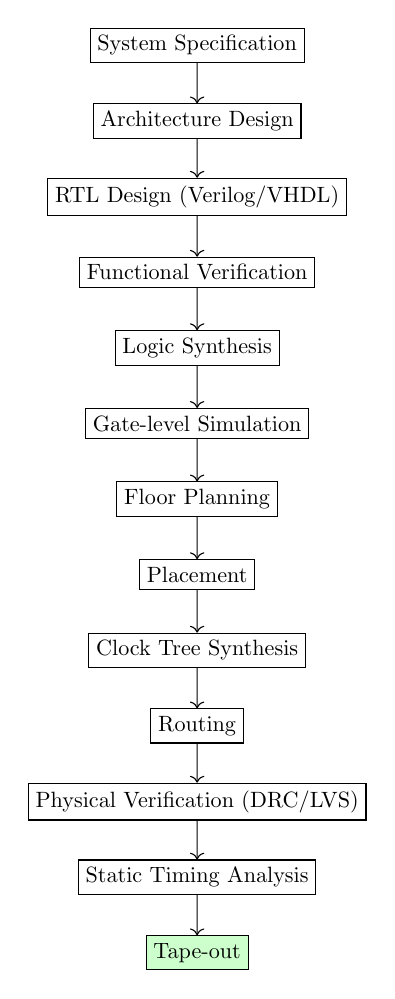
\begin{tikzpicture}[node distance=1.2cm, auto, scale=0.8, transform shape]
    \node (spec) [draw, rectangle, align=center] {System Specification};
    \node (arch) [draw, rectangle, below of=spec] {Architecture Design};
    \node (rtl) [draw, rectangle, below of=arch] {RTL Design (Verilog/VHDL)};
    \node (verif) [draw, rectangle, below of=rtl] {Functional Verification};
    \node (syn) [draw, rectangle, below of=verif] {Logic Synthesis};
    \node (gate) [draw, rectangle, below of=syn] {Gate-level Simulation};
    \node (floor) [draw, rectangle, below of=gate] {Floor Planning};
    \node (place) [draw, rectangle, below of=floor] {Placement};
    \node (cts) [draw, rectangle, below of=place] {Clock Tree Synthesis};
    \node (route) [draw, rectangle, below of=cts] {Routing};
    \node (phys) [draw, rectangle, below of=route] {Physical Verification (DRC/LVS)};
    \node (sta) [draw, rectangle, below of=phys] {Static Timing Analysis};
    \node (tape) [draw, rectangle, below of=sta, fill=green!20] {Tape-out};

    \draw[->] (spec) -- (arch);
    \draw[->] (arch) -- (rtl);
    \draw[->] (rtl) -- (verif);
    \draw[->] (verif) -- (syn);
    \draw[->] (syn) -- (gate);
    \draw[->] (gate) -- (floor);
    \draw[->] (floor) -- (place);
    \draw[->] (place) -- (cts);
    \draw[->] (cts) -- (route);
    \draw[->] (route) -- (phys);
    \draw[->] (phys) -- (sta);
    \draw[->] (sta) -- (tape);
\end{tikzpicture}
\captionof{figure}{ASIC Design Flow}
\end{center}

\textbf{Design Stages:}
\begin{itemize}
    \item \textbf{RTL Design}: Describing hardware behavior using HDL.
    \item \textbf{Synthesis}: Converting RTL to gate-level netlist.
    \item \textbf{Physical Design}: Floorplanning, Placement, and Routing (P\&R).
    \item \textbf{Verification}: ensuring functionality (Functional) and manufacturability (Physical/Timing).
\end{itemize}
\end{solutionbox}

\begin{mnemonicbox}
\mnemonic{ASIC flow: RTL to GDSII}
\end{mnemonicbox}

\questionmarks{4(a)}{3}{Implement the logic function $G = \overline{A(D+E)+BC}$ using CMOS}

\begin{solutionbox}
\textbf{Logic Analysis:}
$G = \overline{A(D+E) + BC}$.
PDN implements $A(D+E) + BC$.
\begin{itemize}
    \item $D+E \rightarrow$ D, E parallel.
    \item $A(D+E) \rightarrow$ A in series with (D parallel E).
    \item $BC \rightarrow$ B, C in series.
    \item Final OR $\rightarrow$ The two branches in parallel.
\end{itemize}

PUN implements dual:
\begin{itemize}
    \item Dual of $(D+E)$ is $D \cdot E$ (series).
    \item Dual of $A(\dots)$ is $A + \dots$ (parallel).
    \item Dual of $BC$ is $B+C$ (parallel).
    \item Dual of major OR is AND (series).
    \item So: $(A \text{ parallel } (D \text{ series } E)) \text{ series } (B \text{ parallel } C)$.
\end{itemize}

\textbf{CMOS Implementation:}

\begin{center}
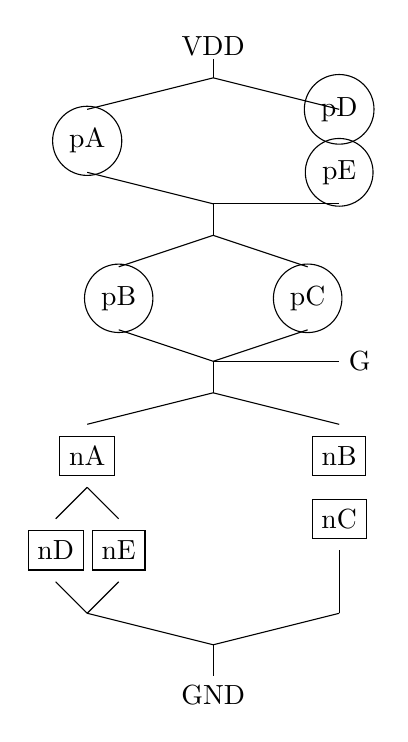
\begin{tikzpicture}[scale=0.8]
    % VDD and PUN
    \node at (0,6) {VDD};
    \draw (0,5.8) -- (0,5.5);
    
    % PUN: (A || (D-E)) --series-- (B || C)
    % Block 1: A || (D-E)
    \draw (0,5.5) -- (-2,5); % To A
    \draw (0,5.5) -- (2,5); % To D-E
    
    \node[draw,circle,minimum size=0.5cm] (pA) at (-2,4.5) {pA};
    \draw (-2,4) -- (0,3.5);
    
    \node[draw,circle,minimum size=0.5cm] (pD) at (2,5) {pD};
    \draw (2,4.5) -- (2,4.5);
    \node[draw,circle,minimum size=0.5cm] (pE) at (2,4) {pE};
    \draw (2,3.5) -- (0,3.5);
    
    % Series connect to Block 2
    \draw (0,3.5) -- (0,3);
    
    % Block 2: B || C
    \draw (0,3) -- (-1.5,2.5);
    \draw (0,3) -- (1.5,2.5);
    
    \node[draw,circle,minimum size=0.5cm] (pB) at (-1.5,2) {pB};
    \node[draw,circle,minimum size=0.5cm] (pC) at (1.5,2) {pC};
    
    \draw (-1.5,1.5) -- (0,1);
    \draw (1.5,1.5) -- (0,1);
    
    % Output Node
    \draw (0,1) -- (2,1) node[right] {G};
    \draw (0,1) -- (0,0.5);
    
    % PDN: (A (D+E) + BC)
    % Branch 1: A series (D || E)
    % Branch 2: B series C
    
    % Parallel split
    \draw (0,0.5) -- (-2,0);
    \draw (0,0.5) -- (2,0);
    
    % Left Branch (A(D+E))
    \node[draw,rectangle,minimum size=0.5cm] (nA) at (-2,-0.5) {nA};
    \draw (-2,-1) -- (-2.5,-1.5);
    \draw (-2,-1) -- (-1.5,-1.5);
    \node[draw,rectangle,minimum size=0.5cm] (nD_n) at (-2.5,-2) {nD};
    \node[draw,rectangle,minimum size=0.5cm] (nE_n) at (-1.5,-2) {nE};
    \draw (-2.5,-2.5) -- (-2,-3);
    \draw (-1.5,-2.5) -- (-2,-3);
    
    % Right Branch (BC)
    \node[draw,rectangle,minimum size=0.5cm] (nB_n) at (2,-0.5) {nB};
    \node[draw,rectangle,minimum size=0.5cm] (nC_n) at (2,-1.5) {nC};
    \draw (2,-2) -- (2,-3);
    
    % Rejoin
    \draw (-2,-3) -- (0,-3.5);
    \draw (2,-3) -- (0,-3.5);
    \draw (0,-3.5) -- (0,-4) node[below] {GND};
\end{tikzpicture}
\captionof{figure}{Complex CMOS Gate}
\end{center}
\end{solutionbox}

\begin{mnemonicbox}
\mnemonic{Complex CMOS - PMOS series, NMOS parallel}
\end{mnemonicbox}

\questionmarks{4(b)}{4}{Write a Verilog code for 3 bit parity checker.}

\begin{solutionbox}
\begin{lstlisting}[language=Verilog]
module parity_checker_3bit(
    input [2:0] data_in,
    output parity_even,
    output parity_odd
);

// Even parity checker
assign parity_even = ^data_in;

// Odd parity checker
assign parity_odd = ~(^data_in);

endmodule
\end{lstlisting}

\textbf{Truth Table:}
\begin{center}
\begin{tabulary}{\linewidth}{|C|C|C|C|}
\hline
\textbf{Input [2:0]} & \textbf{\# of 1s} & \textbf{Even Parity} & \textbf{Odd Parity} \\ \hline
000 & 0 & 0 & 1 \\ \hline
001 & 1 & 1 & 0 \\ \hline
111 & 3 & 1 & 0 \\ \hline
\end{tabulary}
\end{center}
\end{solutionbox}

\questionmarks{4(c)}{7}{Implement: 1) $G = (AD +BC+EF)$ using CMOS [3 marks] 2) $Y' = (ABCD + EF(G+H)+ J)$ using CMOS [4 marks]}

\begin{solutionbox}
\textbf{Part 1: $G = (AD +BC+EF)$ [3 marks]}

\textbf{CMOS Circuit Analysis:}
$G = (AD + BC + EF)$. This is a non-inverting function.
Using strict static CMOS, we implement $\overline{G} = \overline{AD+BC+EF}$ and add an inverter.
PDN for $\overline{G}$ matches the function directly (Parallel branches of Series pairs).

\begin{center}
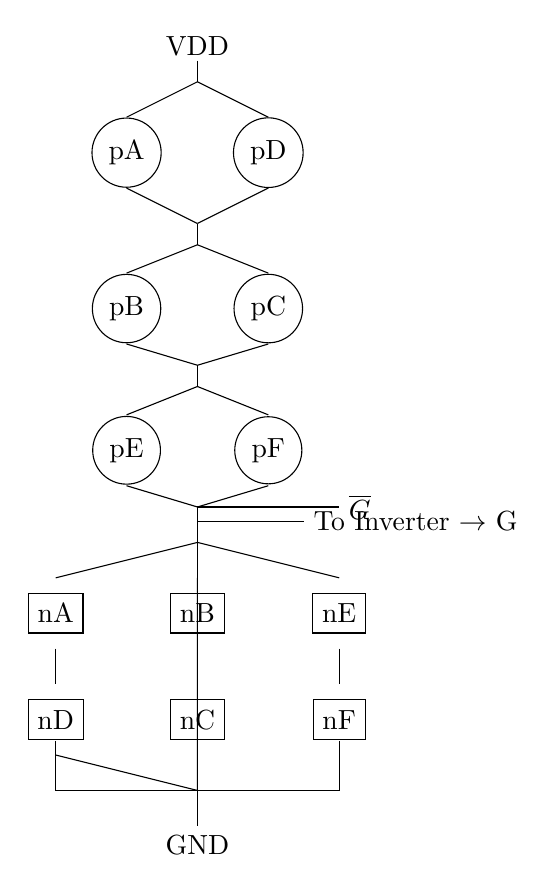
\begin{tikzpicture}[scale=0.9]
    \node at (0,6) {VDD};
    \draw (0,5.8) -- (0,5.5);
    
    % PUN for G_bar: (A+D)(B+C)(E+F)
    % Block 1: A || D
    \draw (0,5.5) -- (-1,5);
    \draw (0,5.5) -- (1,5);
    \node[draw,circle,minimum size=0.5cm] (pA) at (-1,4.5) {pA};
    \node[draw,circle,minimum size=0.5cm] (pD) at (1,4.5) {pD};
    \draw (-1,4) -- (0,3.5);
    \draw (1,4) -- (0,3.5);
    
    % Series to Block 2: B || C
    \draw (0,3.5) -- (0,3.2);
    \draw (0,3.2) -- (-1,2.8);
    \draw (0,3.2) -- (1,2.8);
    \node[draw,circle,minimum size=0.5cm] (pB) at (-1,2.3) {pB};
    \node[draw,circle,minimum size=0.5cm] (pC) at (1,2.3) {pC};
    \draw (-1,1.8) -- (0,1.5);
    \draw (1,1.8) -- (0,1.5);
    
    % Series to Block 3: E || F
    \draw (0,1.5) -- (0,1.2);
    \draw (0,1.2) -- (-1,0.8);
    \draw (0,1.2) -- (1,0.8);
    \node[draw,circle,minimum size=0.5cm] (pE) at (-1,0.3) {pE};
    \node[draw,circle,minimum size=0.5cm] (pF) at (1,0.3) {pF};
    \draw (-1,-0.2) -- (0,-0.5);
    \draw (1,-0.2) -- (0,-0.5);
    
    % Output node
    \draw (0,-0.5) -- (2,-0.5) node[right] {$\overline{G}$};
    \draw (0,-0.5) -- (0,-1);
    \draw (0,-0.7) -- (1,-0.7) -- (1.5,-0.7) node[right]{To Inverter $\rightarrow$ G};
    
    % PDN for G_bar: AD + BC + EF
    \draw (0,-1) -- (-2,-1.5); % Branch 1
    \draw (0,-1) -- (0,-1.5);  % Branch 2
    \draw (0,-1) -- (2,-1.5);  % Branch 3
    
    % Branch 1: A-D
    \node[draw,rectangle,minimum size=0.5cm] (nA) at (-2,-2) {nA};
    \draw (-2,-2.5) -- (-2,-3);
    \node[draw,rectangle,minimum size=0.5cm] (nD_n) at (-2,-3.5) {nD};
    
    % Branch 2: B-C
    \node[draw,rectangle,minimum size=0.5cm] (nB_n) at (0,-2) {nB};
    \draw (0,-2.5) -- (0,-3);
    \node[draw,rectangle,minimum size=0.5cm] (nC_n) at (0,-3.5) {nC};
    
    % Branch 3: E-F
    \node[draw,rectangle,minimum size=0.5cm] (nE_n) at (2,-2) {nE};
    \draw (2,-2.5) -- (2,-3);
    \node[draw,rectangle,minimum size=0.5cm] (nF_n) at (2,-3.5) {nF};
    
    % Rejoin
    \draw (-2,-4) -- (0,-4.5) -- (0,-1.5); 
    \draw (-2,-3.8) -- (-2,-4.5) -- (0,-4.5);
    \draw (0,-3.8) -- (0,-4.5);
    \draw (2,-3.8) -- (2,-4.5) -- (0,-4.5);
    
    \draw (0,-4.5) -- (0,-5) node[below] {GND};
\end{tikzpicture}
\captionof{figure}{CMOS Logic for $G$ (Output $\overline{G}$)}
\end{center}

\textbf{Part 2: $Y' = (ABCD + EF(G+H)+ J)$ [4 marks]}
This requires a complex single stage.
PDN Implementation:
\begin{itemize}
    \item $ABCD$: 4 NMOS in series.
    \item $EF(G+H)$: G parallel H, series with E and F.
    \item $J$: Parallel to everything.
    \item All combined in parallel structure.
\end{itemize}
\end{solutionbox}

\questionmarks{4(a) OR}{3}{Explain AOI logic with example.}

\begin{solutionbox}
\textbf{AOI Definition:}
\textbf{AND-OR-Invert} logic implements functions of form: $Y = \overline{(AB + CD + \dots)}$

\textbf{Example: $Y = \overline{(AB + CD)}$}

\textbf{AOI Implementation:}

\begin{center}
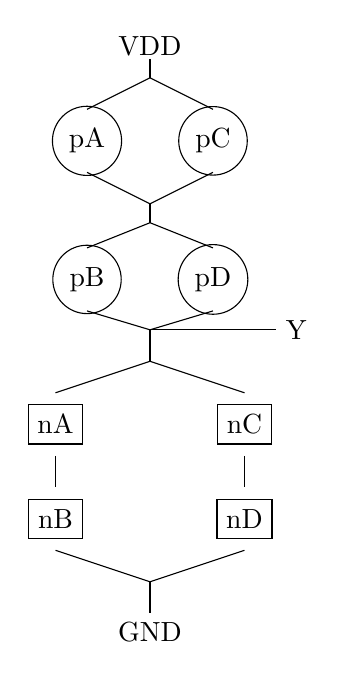
\begin{tikzpicture}[scale=0.8]
    \node at (0,5) {VDD};
    \draw (0,4.8) -- (0,4.5);
    
    % PUN (Dual): (A+B)(C+D)
    \draw (0,4.5) -- (-1,4);
    \draw (0,4.5) -- (1,4);
    \node[draw,circle,minimum size=0.5cm] (pA) at (-1,3.5) {pA};
    \node[draw,circle,minimum size=0.5cm] (pC) at (1,3.5) {pC};
    \draw (-1,3) -- (0,2.5);
    \draw (1,3) -- (0,2.5);
    
    \draw (0,2.5) -- (0,2.2);
    \draw (0,2.2) -- (-1,1.8);
    \draw (0,2.2) -- (1,1.8);
    \node[draw,circle,minimum size=0.5cm] (pB) at (-1,1.3) {pB};
    \node[draw,circle,minimum size=0.5cm] (pD) at (1,1.3) {pD};
    \draw (-1,0.8) -- (0,0.5);
    \draw (1,0.8) -- (0,0.5);
    
    % Output
    \draw (0,0.5) -- (2,0.5) node[right] {Y};
    \draw (0,0.5) -- (0,0);
    
    % PDN: AB + CD
    \draw (0,0) -- (-1.5,-0.5);
    \draw (0,0) -- (1.5,-0.5);
    
    % Branch AB
    \node[draw,rectangle,minimum size=0.5cm] (nA) at (-1.5,-1) {nA};
    \draw (-1.5,-1.5) -- (-1.5,-2);
    \node[draw,rectangle,minimum size=0.5cm] (nB) at (-1.5,-2.5) {nB};
    
    % Branch CD
    \node[draw,rectangle,minimum size=0.5cm] (nC_n) at (1.5,-1) {nC};
    \draw (1.5,-1.5) -- (1.5,-2);
    \node[draw,rectangle,minimum size=0.5cm] (nD_n) at (1.5,-2.5) {nD};
    
    \draw (-1.5,-3) -- (0,-3.5);
    \draw (1.5,-3) -- (0,-3.5);
    \draw (0,-3.5) -- (0,-4) node[below] {GND};
\end{tikzpicture}
\captionof{figure}{AOI Gate Implementation}
\end{center}

\textbf{Advantages:}
\begin{itemize}
    \item \textbf{Single stage}: Direct implementation.
    \item \textbf{Fast}: No propagation through multiple levels.
    \item \textbf{Area efficient}: Fewer transistors than separate gates.
\end{itemize}
\end{solutionbox}

\begin{mnemonicbox}
\mnemonic{AOI - AND-OR-Invert in one stage}
\end{mnemonicbox}

\questionmarks{4(b) OR}{4}{Write Verilog Code for 4-bit Serial IN Parallel out shift register.}

\begin{solutionbox}
\begin{lstlisting}[language=Verilog]
module sipo_4bit(
    input clk,
    input reset,
    input serial_in,
    output reg [3:0] parallel_out
);

always @(posedge clk or posedge reset) begin
    if (reset) begin
        parallel_out <= 4'b0000;
    end else begin
        // Shift left and insert new bit at LSB
        parallel_out <= {parallel_out[2:0], serial_in};
    end
end

endmodule
\end{lstlisting}
\end{solutionbox}

\questionmarks{4(c) OR}{7}{Implement clocked NOR2 SR latch and D-latch using CMOS.}

\begin{solutionbox}
\textbf{Clocked NOR2 SR Latch:}

\begin{center}
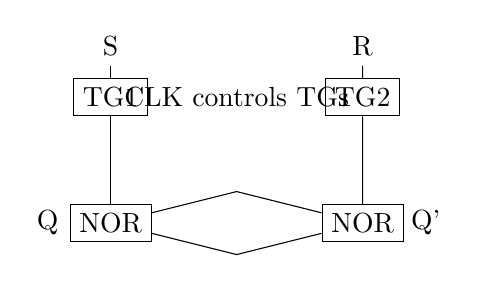
\begin{tikzpicture}[scale=0.8]
    % Transmission Gates
    \node[draw,rectangle] (tg1) at (0,2) {TG1};
    \node[draw,rectangle] (tg2) at (4,2) {TG2};
    \node[above] at (0,2.5) {S};
    \draw (0,2.5) -- (tg1);
    \node[above] at (4,2.5) {R}; 
    \draw (4,2.5) -- (tg2);
    
    % Clock
    \node at (2, 2) {CLK controls TGs};
    
    % Latch Core
    \node[draw,rectangle] (nor1) at (0,0) {NOR};
    \node[draw,rectangle] (nor2) at (4,0) {NOR};
    
    \draw (tg1) -- (nor1);
    \draw (tg2) -- (nor2);
    
    % Feedback
    \draw (nor1) -- (2,-0.5) -- (nor2); % Cross couple simplified
    \draw (nor2) -- (2,0.5) -- (nor1);
    
    \node at (5,0) {Q'};
    \node at (-1,0) {Q};
\end{tikzpicture}
\captionof{figure}{Clocked SR Latch Concept}
\end{center}

\textbf{CMOS D-Latch Circuit:}

\begin{center}
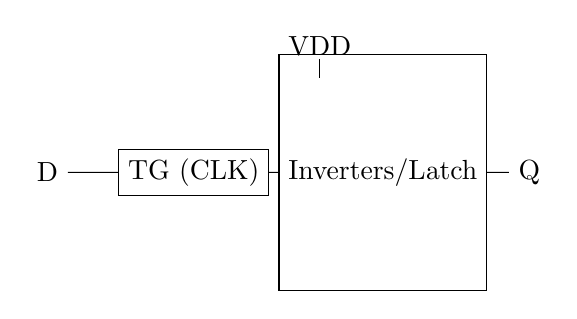
\begin{tikzpicture}[scale=0.8]
    \node at (2,4) {VDD};
    \draw (2,3.8) -- (2,3.5);
    
    % Simplified representation
    \node[draw,rectangle] (tg_in) at (0,2) {TG (CLK)};
    \draw (-2,2) node[left] {D} -- (tg_in);
    
    \node[draw,rectangle,minimum width=2cm, minimum height=3cm] (latch) at (3,2) {Inverters/Latch};
    
    \draw (tg_in) -- (latch);
    \draw (latch) -- (5,2) node[right] {Q};
\end{tikzpicture}
\captionof{figure}{D-Latch}
\end{center}
\end{solutionbox}

\questionmarks{5(a)}{3}{Draw the stick diagram for Y = (PQ +U)' using CMOS considering Euler path approach.}

\begin{solutionbox}
\textbf{Logic Analysis:}
$Y = \overline{PQ + U}$.
PDN: $P \cdot Q + U$ (P series Q, parallel U).
PUN: $\overline{PQ} \cdot \overline{U} = (\bar{P} + \bar{Q}) \cdot \bar{U}$ (P parallel Q, series U).

\textbf{Euler Path:}
Common sequence: \textbf{U - P - Q}.

\textbf{Stick Diagram:}

\begin{center}
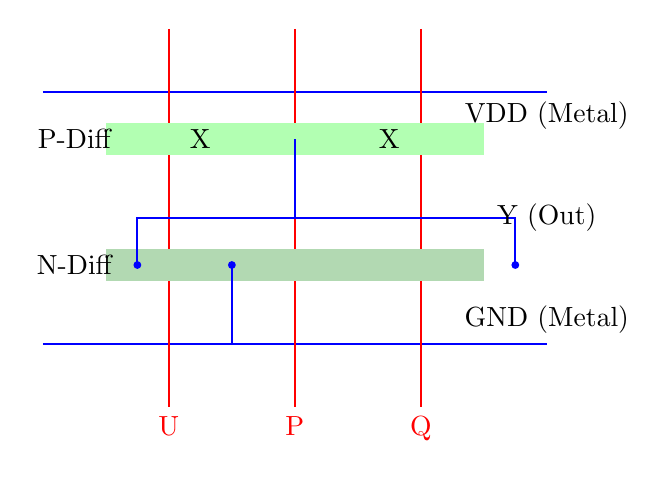
\begin{tikzpicture}[scale=0.8]
    % Rails
    \draw[thick, blue] (0,4) -- (8,4) node[below, black] {VDD (Metal)};
    \draw[thick, blue] (0,0) -- (8,0) node[above, black] {GND (Metal)};
    
    % Polysilicon Gates
    \draw[thick, red] (2,5) -- (2,-1) node[below] {U};
    \draw[thick, red] (4,5) -- (4,-1) node[below] {P};
    \draw[thick, red] (6,5) -- (6,-1) node[below] {Q};
    
    % P-Diffusion (PUN)
    \fill[green!30] (1,3) rectangle (7,3.5);
    \node at (0.5,3.25) {P-Diff};
    
    % N-Diffusion (PDN)
    \fill[green!50!black!30] (1,1) rectangle (7,1.5);
    \node at (0.5,1.25) {N-Diff};
    
    % Metal connections (X)
    \draw[thick, blue] (3,1.25) node[circle,fill,inner sep=1pt]{} -- (3,0); 
    \draw[thick, blue] (1.5,1.25) node[circle,fill,inner sep=1pt]{} -- (1.5,2) -- (4,2) -- (4,2.5) -- (4,3.25); 
    \draw[thick, blue] (7.5,1.25) node[circle,fill,inner sep=1pt]{} -- (7.5,2) -- (4,2); 
    
    % Contacts
    \node at (2.5,3.25) {X}; 
    \node at (5.5,3.25) {X}; 
    
    % Output
    \node at (8,2) {Y (Out)};
    
\end{tikzpicture}
\captionof{figure}{Stick Diagram for Y}
\end{center}
\end{solutionbox}

\begin{mnemonicbox}
\mnemonic{Stick diagram shows physical layout with Euler path optimization}
\end{mnemonicbox}

\questionmarks{5(b)}{4}{Implement 8x1 multiplexer using Verilog.}

\begin{solutionbox}
\begin{lstlisting}[language=Verilog]
module mux_8x1(
    input [7:0] data_in,
    input [2:0] select,
    output reg data_out
);

always @(*) begin
    case (select)
        3'b000: data_out = data_in[0];
        3'b001: data_out = data_in[1];
        3'b010: data_out = data_in[2];
        3'b011: data_out = data_in[3];
        3'b100: data_out = data_in[4];
        3'b101: data_out = data_in[5];
        3'b110: data_out = data_in[6];
        3'b111: data_out = data_in[7];
        default: data_out = 1'b0;
    endcase
end

endmodule
\end{lstlisting}
\end{solutionbox}

\questionmarks{5(c)}{7}{Implement full adder using behavioral modeling style in Verilog.}

\begin{solutionbox}
\begin{lstlisting}[language=Verilog]
module full_adder_behavioral(
    input A,
    input B,
    input Cin,
    output reg Sum,
    output reg Cout
);

always @(*) begin
    case ({A, B, Cin})
        3'b000: begin Sum = 0; Cout = 0; end
        3'b001: begin Sum = 1; Cout = 0; end
        3'b010: begin Sum = 1; Cout = 0; end
        3'b011: begin Sum = 0; Cout = 1; end
        3'b100: begin Sum = 1; Cout = 0; end
        3'b101: begin Sum = 0; Cout = 1; end
        3'b110: begin Sum = 0; Cout = 1; end
        3'b111: begin Sum = 1; Cout = 1; end
        default: begin Sum = 0; Cout = 0; end
    endcase
end

endmodule
\end{lstlisting}
\end{solutionbox}

\questionmarks{5(a) OR}{3}{Implement NOR2 gate CMOS circuit with its stick diagram.}

\begin{solutionbox}
\textbf{CMOS NOR2 Circuit:}

\begin{center}
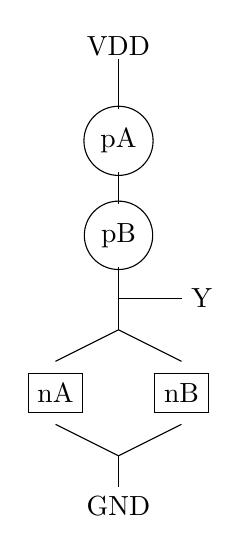
\begin{tikzpicture}[scale=0.8]
    \node at (0,4) {VDD};
    \draw (0,3.8) -- (0,3.5);
    
    % Logic: Y = (A+B)'. PDN: A || B. PUN: A series B.
    
    % PUN
    \draw (0,3.5) -- (0,3);
    \node[draw,circle,minimum size=0.5cm] (pA) at (0,2.5) {pA};
    \draw (0,2) -- (0,1.5);
    \node[draw,circle,minimum size=0.5cm] (pB) at (0,1) {pB};
    \draw (0,0.5) -- (0,0); 
    
    \draw (0,0) -- (1,0) node[right] {Y};
    \draw (0,0) -- (0,-0.5);
    
    % PDN
    \draw (0,-0.5) -- (-1,-1);
    \draw (0,-0.5) -- (1,-1);
    
    \node[draw,rectangle,minimum size=0.5cm] (nA) at (-1,-1.5) {nA};
    \node[draw,rectangle,minimum size=0.5cm] (nB) at (1,-1.5) {nB};
    
    \draw (-1,-2) -- (0,-2.5);
    \draw (1,-2) -- (0,-2.5);
    \draw (0,-2.5) -- (0,-3) node[below] {GND};
\end{tikzpicture}
\captionof{figure}{CMOS NOR2 Circuit}
\end{center}

\textbf{Stick Diagram:}

\begin{center}
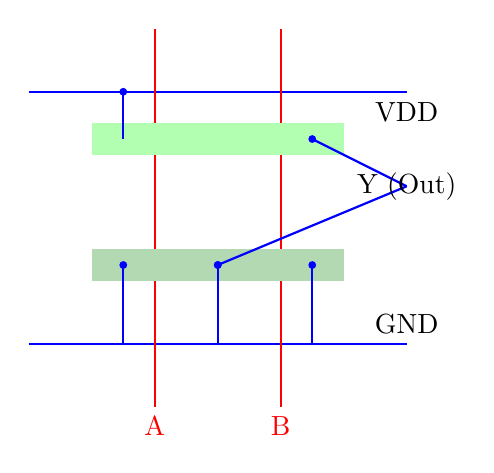
\begin{tikzpicture}[scale=0.8]
    % Rails
    \draw[thick, blue] (0,4) -- (6,4) node[below, black] {VDD};
    \draw[thick, blue] (0,0) -- (6,0) node[above, black] {GND};
    
    % Gates
    \draw[thick, red] (2,5) -- (2,-1) node[below] {A};
    \draw[thick, red] (4,5) -- (4,-1) node[below] {B};
    
    % PUN (Series)
    \fill[green!30] (1,3) rectangle (5,3.5);
    
    % PDN (Parallel)
    \fill[green!50!black!30] (1,1) rectangle (5,1.5);
    
    % Connections
    \draw[thick, blue] (1.5,4) node[circle,fill,inner sep=1pt]{} -- (1.5,3.25); % VDD to pA source
    \draw[thick, blue] (3,1.25) node[circle,fill,inner sep=1pt]{} -- (3,0); 
    
    % Correct wiring for Euler Path A-B
    % PUN
    \draw[thick, blue] (1.5,3.25) -- (1.5,4); % VDD left of A
    \draw[thick, blue] (4.5,3.25) node[circle,fill,inner sep=1pt]{} -- (6,2.5); % Out right of B
    
    % PDN
    \draw[thick, blue] (1.5,1.25) node[circle,fill,inner sep=1pt]{} -- (1.5,0); % GND left of A
    \draw[thick, blue] (4.5,1.25) node[circle,fill,inner sep=1pt]{} -- (4.5,0); % GND right of B
    \draw[thick, blue] (3,1.25) node[circle,fill,inner sep=1pt]{} -- (6,2.5); % Out between A and B
    
    \node at (6,2.5) {Y (Out)};
\end{tikzpicture}
\captionof{figure}{NOR2 Stick Diagram}
\end{center}
\end{solutionbox}

\questionmarks{5(b) OR}{4}{Implement 4 bit up counter using Verilog}

\begin{solutionbox}
\begin{lstlisting}[language=Verilog]
module counter_4bit_up(
    input clk,
    input reset,
    input enable,
    output reg [3:0] count
);

always @(posedge clk or posedge reset) begin
    if (reset) begin
        count <= 4'b0000;
    end else if (enable) begin
        if (count == 4'b1111) begin
            count <= 4'b0000;
        end else begin
            count <= count + 1;
        end
    end
end

endmodule
\end{lstlisting}
\end{solutionbox}

\questionmarks{5(c) OR}{7}{Implement 3:8 decoder using behavioral modeling style in Verilog.}

\begin{solutionbox}
\begin{lstlisting}[language=Verilog]
module decoder_3x8_behavioral(
    input [2:0] address,
    input enable,
    output reg [7:0] decode_out
);

always @(*) begin
    if (enable) begin
        case (address)
            3'b000: decode_out = 8'b00000001; 
            3'b001: decode_out = 8'b00000010; 
            3'b010: decode_out = 8'b00000100;
            3'b011: decode_out = 8'b00001000;
            3'b100: decode_out = 8'b00010000;
            3'b101: decode_out = 8'b00100000;
            3'b110: decode_out = 8'b01000000;
            3'b111: decode_out = 8'b10000000;
            default: decode_out = 8'b00000000;
        endcase
    end else begin
        decode_out = 8'b00000000;
    end
end

endmodule
\end{lstlisting}
\end{solutionbox}

\end{document}
